\documentclass[mathserif, serif]{beamer}

%\documentclass[a4paper,11pt,onecolumn,twoside,openright,titlepage]{article}

\usepackage[T1]{fontenc}
\usepackage[polish]{babel}
\usepackage[utf8]{inputenc}
\usepackage{lmodern}
\usepackage{amsmath}
\usepackage[T1]{fontenc}
\usepackage[polish]{babel}
\usepackage[utf8]{inputenc}
\usepackage{lmodern}
\usepackage{hyperref}
\usepackage{float}
\usepackage{changepage}
\usepackage{pdflscape}
\usepackage{multirow}
\usepackage{tabularx}
\usepackage{array}
\usepackage{algorithmic}
\usepackage{tikz}
\usetikzlibrary{positioning}
\usetikzlibrary{arrows}
\usetikzlibrary{shapes}
\usepackage{pgfplots}
\usetikzlibrary{decorations.pathreplacing}
\selectlanguage{polish}
\usetikzlibrary{arrows.meta}

\author{Aleksander Sas}
\title{Rozpoznawanie mowy}
\usetheme{Warsaw}

\DeclareMathOperator*{\argmax}{\arg\max}   % rbp
\tikzstyle{hmm0}=[circle,thick,draw=gray!50,fill=gray!13,minimum size=4mm]
\tikzstyle{hmm}=[circle,thick,draw=gray!75,fill=gray!20,minimum size=6mm]
\tikzstyle{line} = [draw, -latex']


\begin{document}
	\begin{frame}
		\titlepage
	\end{frame}

	\begin{frame}
		\frametitle{Etapy rozpoznawania mowy}
		
		\begin{figure}
			\scalebox{.65}{
				\begin{tikzpicture}[node distance = 1.7cm, auto]
				
				\tikzstyle{ArmBlok} = [rectangle, draw, fill=blue!20, text width=12em, text centered, rounded corners, minimum height=3em]
				\tikzstyle{model} = [ellipse, draw, fill=blue!20, text width=7em, text centered, rounded corners, minimum height=3em, node distance=5cm]
				\tikzstyle{data} = [draw, ellipse,fill=red!20, node distance=2cm,minimum height=2em]
				
				% Place nodes
				\node [data] (etap0) {Mowa};
				\node [ArmBlok,  below of=etap0] (etap1) {Zbieranie sygnału akustycznego};
				\node [ArmBlok,  below of=etap1] (etap2) { Ekstrakcja cech};
				\node [ArmBlok,  below of=etap2, fill=blue!40] (etap3) {Klasyfikacja stanów};
				\node [ArmBlok,  below of=etap3] (etap4) { Wyszukiwanie najlepszej ścieżki w modelu Markowa};
				\node [model, right of=etap3] (etap5) { Model językowy};
				\node [model,    left  of=etap2, fill=blue!40] (model_akustyczny) { Model akustyczny};
				\node [data,     below of=etap4] (etap6) {Rozpoznanie};
				\node [model,   right  of=etap6] (slownik) {Słownik};
				
				\path [line] (etap0) -- (etap1);
				\path [line] (etap1) -- (etap2);
				\path [line] (etap2) -- (etap3);
				\path [line] (etap3) -- (etap4);
				\path [line, dashed] (etap5) |- (etap4);
				\path [line] (etap4) -- (etap6);
				\path [line, dashed] (slownik) |- (etap4);
				\path [line, dashed] (model_akustyczny) |- (etap3);
				\path [line, dashed] (model_akustyczny) |- (etap4);
				
				\end{tikzpicture}
			}
		\end{figure}
	\end{frame}	

	\begin{frame}
		\frametitle{Model fonemu}
		
			\begin{itemize}
				\item Fonemy reprezentują dźwięki.
				\item Modelujemy je trzema stanami modelu Markowa.
				\item Dźwięki mogą mieć różną długość.
				\item Trifony są rozwinięciem koncepcji fonów, przykładowo $a-g+r$.
			\end{itemize}		
		
		\begin{figure}
			\scalebox{.8}{
				\begin{tikzpicture}[node distance=1.7cm]
				
				\begin{scope}
				\node [hmm] (hmm1) {$s_1$};
				\node [hmm, right of=hmm1] (hmm2) {$s_2$};
				\node [hmm, right of=hmm2] (hmm3) {$s_2$};
				
				\draw[thick,->,shorten >=1pt] (hmm1) to [out=0,in=180] (hmm2);
				\draw[thick,->,shorten >=1pt] (hmm2) to [out=0,in=180] (hmm3);
				
				\draw[thick,->] (hmm1.70) arc (-60:245:4mm);
				\draw[thick,->] (hmm2.70) arc (-60:245:4mm);
				\draw[thick,->] (hmm3.70) arc (-60:245:4mm);
				
				\draw[thick,<-,shorten <=1pt] (hmm1) -- +(180:1cm);
				\draw[thick,->,shorten <=1pt] (hmm3) -- +(0:1cm);
				\end{scope}
				
				\end{tikzpicture}
			}
		\end{figure}
	\end{frame}

	\begin{frame}
		\frametitle{Fonemy modelowane w systemie}
		
		\begin{itemize}
			\item Zamodelowano 40 fonemów.
			\item $40\times40\times40=64000$ możliwych trifonów.
			\item W praktyce wystąpiło 27005 różnych trifonów.
		\end{itemize}		
		
		\begin{table}
			\begin{tabular}{|c c c c c c c c|}
				\hline
				a  & o\~ & b & c & cz & ć & d & dz \\ 
				dź & dż & e & e\~ & f & g & g\^ & h \\
				i & j & k & k\^ & l & ł & m & n \\
				nn & ń & o & p  & r & s & sz & ś \\
				t & u & v & y & z & ź & ż & sil \\
				\hline
			\end{tabular}
		\end{table}
	\end{frame}

	\begin{frame}
		\frametitle{składanie fonemów}
		
		\begin{figure}[H]
			\centering
			\begin{tabular}{|c|}
				\hline
				\textit{jabłko} = [j a p ł k o] \\ 
				\hline \\
				
				\begin{tikzpicture}[node distance=1.7cm]
				
				\begin{scope}
				
				\def\x{0.65}
				\def\y{1.0}
				\def\z{2.5}
				
				\node [hmm0] (hmm1) {};
				\node [below] at (hmm1.south) {$j_1$};
				
				\node [hmm0, right = \x cm of hmm1] (hmm2) {};
				\node [below] at (hmm2.south) {$j_2$};
				
				\node [hmm0, right = \x cm of hmm2] (hmm3) {};
				\node [below] at (hmm3.south) {$j_3$};
				
				
				\node [hmm0, right = \y cm of hmm3] (hmm4) {};
				\node [below] at (hmm4.south) {$a_1$};
				
				\node [hmm0, right = \x cm of hmm4] (hmm5) {};
				\node [below] at (hmm5.south) {$a_2$};
				
				\node [hmm0, right = \x cm of hmm5] (hmm6) {};
				\node [below] at (hmm6.south) {$a_3$};
				
				
				\node [hmm0, right = \y cm of hmm6] (hmm7) {};
				\node [below] at (hmm7.south) {$p_1$};
				
				\node [hmm0, right = \x cm of hmm7] (hmm8) {};
				\node [below] at (hmm8.south) {$p_2$};
				
				\node [hmm0, right = \x cm of hmm8] (hmm9) {};
				\node [below] at (hmm9.south) {$p_3$};
				
				
				
				
				\node [hmm0, below = \z cm of hmm9] (hmm10) {};
				\node [below] at (hmm10.south) {$\text{\textit{ł}}_1$};
				
				\node [hmm0, left = \x cm of hmm10] (hmm11) {};
				\node [below] at (hmm11.south) {$\text{\textit{ł}}_2$};
				
				\node [hmm0, left = \x cm of hmm11] (hmm12) {};
				\node [below] at (hmm12.south) {$\text{\textit{ł}}_3$};
				
				
				\node [hmm0, left = \y cm of hmm12] (hmm13) {};
				\node [below] at (hmm13.south) {$k_1$};
				
				\node [hmm0, left = \x cm of hmm13] (hmm14) {};
				\node [below] at (hmm14.south) {$k_2$};
				
				\node [hmm0, left = \x cm of hmm14] (hmm15) {};
				\node [below] at (hmm15.south) {$k_3$};
				
				
				\node [hmm0, left = \y cm of hmm15] (hmm16) {};
				\node [below] at (hmm16.south) {$o_1$};
				
				\node [hmm0, left = \x cm of hmm16] (hmm17) {};
				\node [below] at (hmm17.south) {$o_2$};
				
				\node [hmm0, left = \x cm of hmm17] (hmm18) {};
				\node [below] at (hmm18.south) {$o_3$};
				
				
				
				\draw[thick,->,shorten >=1pt] (hmm1) to [out=0,in=180] (hmm2);
				\draw[thick,->,shorten >=1pt] (hmm2) to [out=0,in=180] (hmm3);
				
				\draw[thick,->,shorten >=1pt] (hmm3) to [out=0,in=180] (hmm4);
				
				\draw[thick,->,shorten >=1pt] (hmm4) to [out=0,in=180] (hmm5);
				\draw[thick,->,shorten >=1pt] (hmm5) to [out=0,in=180] (hmm6);
				
				\draw[thick,->,shorten >=1pt] (hmm6) to [out=0,in=180] (hmm7);
				
				\draw[thick,->,shorten >=1pt] (hmm7) to [out=0,in=180] (hmm8);
				\draw[thick,->,shorten >=1pt] (hmm8) to [out=0,in=180] (hmm9);
				
				\draw[thick,->,shorten >=1pt] (hmm9) to [out=0,in=0,looseness=1.1] (hmm10);
				
				\draw[thick,->,shorten >=1pt] (hmm10) to [out=180,in=0] (hmm11);
				\draw[thick,->,shorten >=1pt] (hmm11) to [out=180,in=0] (hmm12);
				
				\draw[thick,->,shorten >=1pt] (hmm12) to [out=180,in=0] (hmm13);
				
				\draw[thick,->,shorten >=1pt] (hmm13) to [out=180,in=0] (hmm14);
				\draw[thick,->,shorten >=1pt] (hmm14) to [out=180,in=0] (hmm15);
				
				\draw[thick,->,shorten >=1pt] (hmm15) to [out=180,in=0] (hmm16);
				
				\draw[thick,->,shorten >=1pt] (hmm16) to [out=180,in=0] (hmm17);
				\draw[thick,->,shorten >=1pt] (hmm17) to [out=180,in=0] (hmm18);
				
				
				\draw[thick,->] (hmm1.70) arc (-60:245:4mm);
				\draw[thick,->] (hmm2.70) arc (-60:245:4mm);
				\draw[thick,->] (hmm3.70) arc (-60:245:4mm);
				
				\draw[thick,->] (hmm4.70) arc (-60:245:4mm);
				\draw[thick,->] (hmm5.70) arc (-60:245:4mm);
				\draw[thick,->] (hmm6.70) arc (-60:245:4mm);
				
				\draw[thick,->] (hmm7.70) arc (-60:245:4mm);
				\draw[thick,->] (hmm8.70) arc (-60:245:4mm);
				\draw[thick,->] (hmm9.70) arc (-60:245:4mm);
				
				
				
				\draw[thick,->] (hmm10.110) arc (240:-65:4mm);
				\draw[thick,->] (hmm11.110) arc (240:-65:4mm);
				\draw[thick,->] (hmm12.110) arc (240:-65:4mm);
				
				\draw[thick,->] (hmm13.110) arc (240:-65:4mm);
				\draw[thick,->] (hmm14.110) arc (240:-65:4mm);
				\draw[thick,->] (hmm15.110) arc (240:-65:4mm);
				
				\draw[thick,->] (hmm16.110) arc (240:-65:4mm);
				\draw[thick,->] (hmm17.110) arc (240:-65:4mm);
				\draw[thick,->] (hmm18.110) arc (240:-65:4mm);
				
				\draw[thick,<-,shorten <=1pt] (hmm1) -- +(180:1cm);
				\draw[thick,->,shorten <=1pt] (hmm18) -- +(180:1cm);
				\end{scope}			
				\end{tikzpicture} \\
				
				\hline
			\end{tabular}
			\caption{Automat dla słowa \textit{jabłko}}
		\end{figure}
	\end{frame}

	\begin{frame}
		\frametitle{MFCC}
		\footnotesize
		
		\begin{itemize}
			\item Podział ygnału akustycznego na ramki 25ms.
			\item Transformata Fouriera.
			\item Nałożenie zestawu filtrów MEL-owych.
			\item Nałożenie logarytmu.
			\item Dyskretna transformata kosinusowa. 
			\item Typowo 39-cio wymiarowe rozkłady (12 filtrów + calkowita energia) x (0,1,2 pochodna).
		\end{itemize}
	
	\end{frame}

	\begin{frame}
		\frametitle{MFCC}
		\footnotesize
		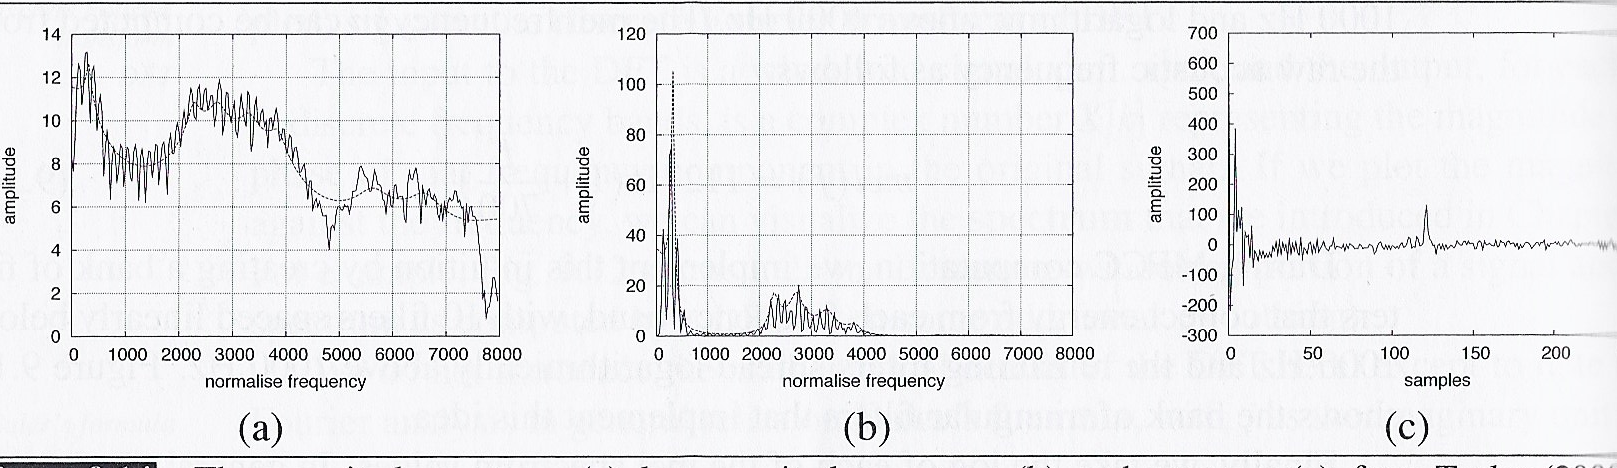
\includegraphics[scale=0.3, trim=3cm 0 0 0cm]{sound}
	\end{frame}

	\begin{frame}
		\frametitle{MFCC}
		\footnotesize
		
		\begin{equation}
		H_m(x)= 
		\begin{cases}
		0,				 					 & x < f(m-1) 		       \\
		\frac{x - f(m-1)}{\big(f(m) - f(m-1)\big)^2}, & f(m-1) \leq x \leq f(m) \\
		\frac{f(m+1) - k}{\big(f(m+1) - f(m)\big)^2}, & f(m) \leq x \leq f(m+1) \\
		0,				 					 & x > f(m+1)
		\end{cases}
		\label{eqn:filter}
		\end{equation}
		
		\begin{figure}[H]
			\centering
			\begin{tikzpicture}[node distance=1.7cm]
			
			\begin{scope}
			
			\def\q{2.8};
			\def\w{3.5}
			
			\draw[-stealth] (0cm,0cm)--(9.4cm,0cm) node[right]{Hz}; 
			\draw[-stealth] (0cm,0cm)--(0cm,\q cm); 
			
			\def\a{0.15}; \node at (\a, -0.5) {f(1)};
			\def\s{1.0};  \node at (\s, -0.5) {f(2)};
			\def\d{2.0};  \node at (\d, -0.5) {f(3)};
			\def\f{3.6};  \node at (\f, -0.5) {f(4)};
			\def\g{5.8};  \node at (\g, -0.5) {f(5)};
			\def\h{8.8};  \node at (\h, -0.5) {f(6)};
			
			\path [line, dashed] (\s, 1.0) -- (\s, \w) node[above] {$v_1$};
			\path [line, dashed] (\d, 1.0) -- (\d, \w) node[above] {$v_2$};
			\path [line, dashed] (\f, 1.0) -- (\f, \w) node[above] {$v_3$}; 
			\path [line, dashed] (\g, 1.0) -- (\g, \w) node[above] {$v_4$};
			
			\pgfmathsetmacro{\z}{1.0 * \q / (\d - \a) * (\d - \a)};
			\draw[-] (\a cm,0cm)--(\s cm,\z cm); 
			\draw[-] (\d cm,0.0cm)--(\s cm,\z cm); 
			
			\pgfmathsetmacro{\z}{1.0 * \q / (\f - \s) * (\d - \a)};
			\draw[-] (\s cm,0.0cm)--(\d cm,\z cm); 
			\draw[-] (\f cm,0.0cm)--(\d cm,\z cm); 
			
			\pgfmathsetmacro{\z}{1.0 * \q / (\g - \d) * (\d - \a)};
			\draw[-] (\d cm,0cm)--(\f cm,\z cm); 
			\draw[-] (\g cm,0.0cm)--(\f cm,\z cm); 
			
			\pgfmathsetmacro{\z}{1.0 * \q / (\h - \f) * (\d - \a)};
			\draw[-] (\f cm,0cm)--(\g cm,\z cm); 
			\draw[-] (\h cm,0.0cm)--(\g cm,\z cm);
			
			\end{scope}
			
			\end{tikzpicture}
			\caption{Wizualizacja $4$ kolejnych filtrów trójkątnych.}
			\label{fig:filter_bank}
			
		\end{figure}
	\end{frame}

	\begin{frame}
		\frametitle{Mikstury Gaussowskie}
		\footnotesize
		\begin{itemize}
			\item Dla każdej ramki (wektora cech) potrzebujemy $P(o|s)$.
			\item W przyrodzie wszystko ma rozkład Gaussowski.
			\item Typowo 39-cio wymiarowe rozkłady.
		\end{itemize}
		
		\begin{figure}
			\scalebox{.8}{
				\begin{tikzpicture}
				\begin{axis}[
				axis lines = left
				]
				%Below the red parabola is defined
				\addplot [
				domain=0:20, 
				samples=100, 
				color=red,
				]
				{0.3 * 1/(2.5 * 2) * e ^ (-(x - 5)^2 / (2 * 2 ^ 2))};
				
				\addplot [
				domain=0:20, 
				samples=100, 
				color=blue,
				]
				{0.3 * 1/(2.5 * 4) * e ^ (-(x - 17)^2 / (2 * 4 ^ 2))};
				
				\addplot [
				domain=0:20, 
				samples=100, 
				color=yellow,
				]
				{0.4 * 1/(2.5 * 1.5) * e ^ (-(x - 10)^2 / (2 * 1.5 ^ 2))};
				
				\addplot [
				domain=0:20, 
				samples=100, 
				color=black,
				]
				{0.3 * 1/(2.5 * 2) * e ^ (-(x - 5)^2 / (2 * 2 ^ 2)) + 0.3 * 1/(2.5 * 4) * e ^ (-(x - 17)^2 / (2 * 4 ^ 2)) + 0.4 * 1/(2.5 * 1.5) * e ^ (-(x - 10)^2 / (2 * 1.5 ^ 2))};
				
				\end{axis}
				\end{tikzpicture}
			}
		\end{figure}
	\end{frame}

	\begin{frame}
		\frametitle{Mikstury Gaussowskie}
		\footnotesize
		
		\begin{equation}
				P(o|s_j)=b_j(o) = \sum_{m=1}^N c_{j,m} N_{j,m}(o)
				\label{eqn:GMM}
		\end{equation}
		\begin{equation}
			N_{j,m}(o)=\frac{1}{(2\pi)^{\frac{D}{2}}||\Sigma_{j,m}|^{\frac{1}{2}}}\exp\bigg( -\frac{1}{2}(o-\mu_{j,m})^T\Sigma_{j,m}^{-1}(o-\mu_{j,m}) \bigg)
			\label{eqn:normal_distribution}
		\end{equation}	
		\begin{equation}
			N_{j,m}(o)\simeq\frac{1}{(2\pi)^{\frac{D}{2}}(\prod_{i=1}^D\sigma_{j,m,i})^{\frac{1}{2}}}\exp\bigg( -\frac{1}{2}\sum_{i=1}^D(o_i-\mu_{j,m,i})^2\sigma_{j,m,i} \bigg)
			\label{eqn:normal_distribution_simple}
		\end{equation}
		
	\end{frame}

	\begin{frame}
		\frametitle{Ukryty Model Markowva}
		\footnotesize
		
		\begin{equation}
		HMM = (Q, O, A, B, q_0, q_F)
		\label{equation:HMM_def}
		\end{equation}
		gdzie
		\begin{align*}
		\mathbf{Q}=\{q_1, q_2,\ldots,q_n\} & &&  \text{Zbiór stanów automatu} \\
		\mathbf{O}=\{o_1, o_2,\ldots,o_k\} & &&  \text{Zbiór obserwacji} \\
		\mathbf{A} =
		\left| \begin{array}{ccc}
		a_{1,1} & \ldots & a_{1,n} \\
		\vdots  & \ddots & \vdots\\
		a_{n,1} & \ldots & a_{n,n}
		\end{array} \right|
		& &&  \text{Macierz przejścia pomiędzy stanami} \\
		& && \\
		\mathbf{B}=\{B_1(o),\ldots,B_n(o)\},o \in O & && \text{zbiór rozkładów prawdopodobieństwa emisji} \\ 
		& && \text{obserwacji \textit{o} w stanie \textit{i}} \\
		\mathbf{q_0, q_F}				  & && \text{stany początkowy i końcowy}
		\end{align*}
	\end{frame}

	\begin{frame}
		\frametitle{Ukryty Model Markowa - przykład}
		\footnotesize
		
		\begin{itemize}
			\item Q=\{dzien\_cieply, dzien\_zimny\} Zbiór stanów automatu
			\item O=\{1, 2, 3\}   Zbiór obserwacji - zjedzonych lodow
			\item F=\{1, 1, 1, 3\}  Zaobserwowane zdarzenia
		\end{itemize}
		\text{Jaki jest najbardziej prawdopodobny ciąg dni?}
		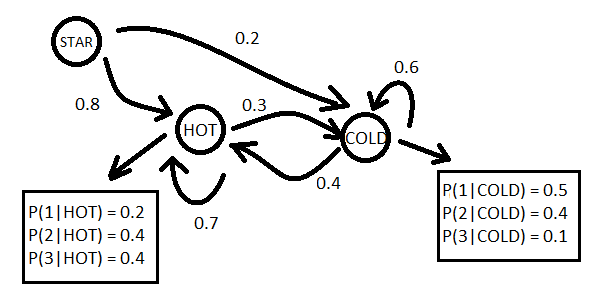
\includegraphics[scale=0.5]{hmm}
		\text{Odp: zimny, zimny, zimny, ciepły}
	\end{frame}

	\begin{frame}
		\frametitle{Model językowy}
		\footnotesize
		
		\begin{itemize}
			\item N-gramowy model jezykowy
			\item Typowo 2-gramowy
			\item Smoothing (Add-one, Kat)
			\item Uczone na korpusach (np medyczny, prawny)
		\end{itemize}
	
		\begin{center}
			$P(w_i|w_{i-1},w_{i-2},\cdots,w_{i-n})$.
		\end{center}
	\end{frame}

	\begin{frame}
		\frametitle{Rozpoznawanie mowy}
		\footnotesize
		
		\begin{equation}
			\hat{W}=\argmax_{W \in \Sigma^{*}}{P(W \mid O)} = \argmax_{W \in \Sigma^{*}}{\frac{P(O \mid W)P(W)}{P(O)}} = \argmax_{W \in \Sigma^{*}}{P(O \mid W)P(W)}
			\label{equation:ASR_definicja2}
		\end{equation}
	\end{frame}

	\begin{frame}
		\frametitle{Graf przejsc}
		\footnotesize
		
		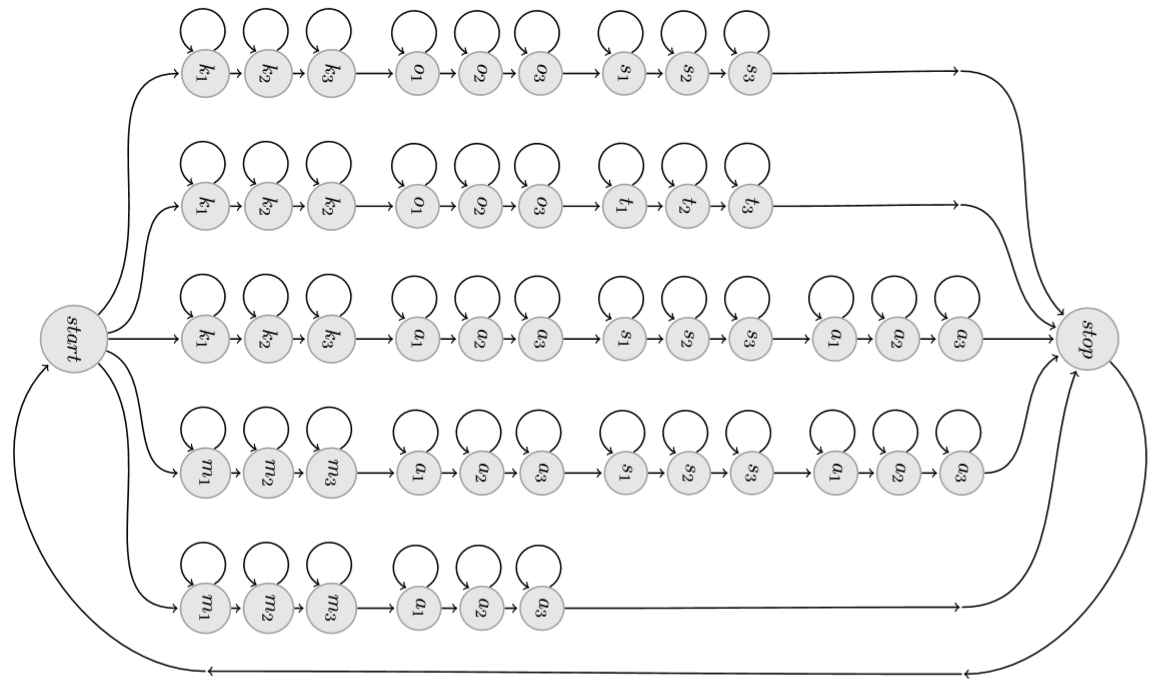
\includegraphics[scale=0.4, trim=2cm 0 0 0cm]{tree1}
	\end{frame}

	\begin{frame}
		\frametitle{Graf przejsc}
		\footnotesize
		
		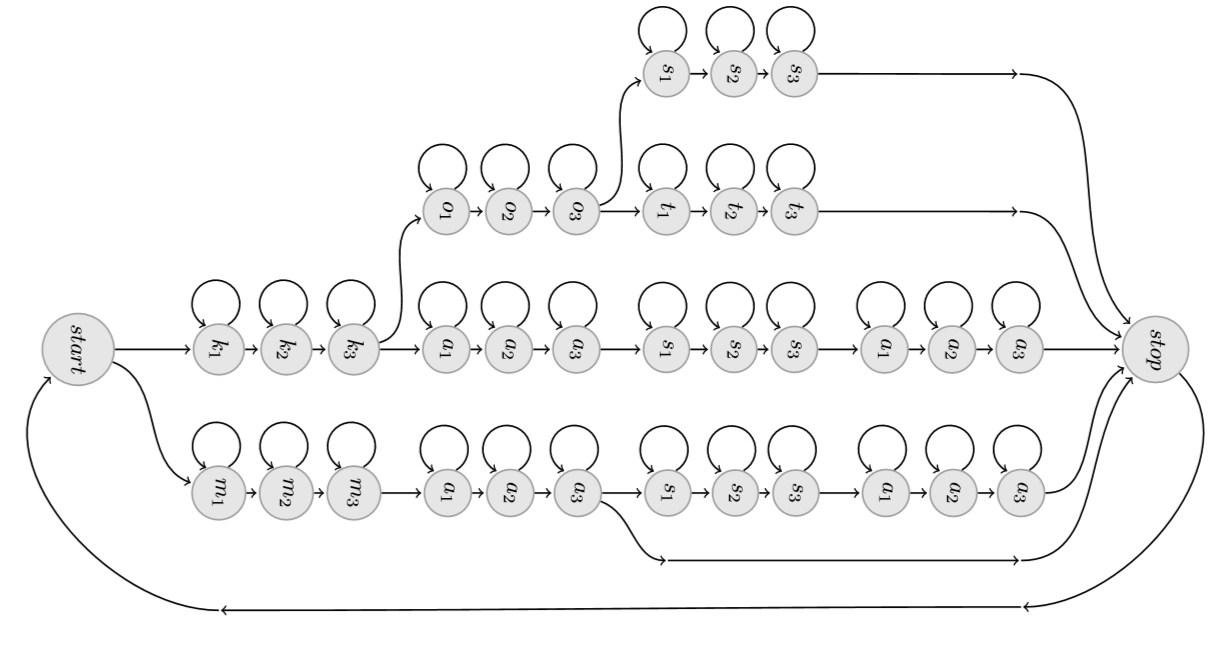
\includegraphics[scale=0.39, trim=3cm 0 0 0cm]{tree2}
	\end{frame}
	
	\begin{frame}
		\frametitle{Token passing}
		\footnotesize
		
		\begin{figure}			
			\begin{tikzpicture}[node distance=2.5cm]
			\begin{scope} 		
			\node at (2.0,4.3){$t=n$};
			\node at (9.0,4.3){$t=n+1$};
			
			\node at (1.0,-2.0){$P(0_{t+1}|k_3)=0.1$};
			\node at (1.0,-2.5){$P(0_{t+1}|a_1)=0.5$};
			\node at (1.0,-3.0){$P(0_{t+1}|u_1)=0.1$};
			
			\node [hmm, fill=red!20] (hmm1) at (0,0) {$k_3$}; \node [below, red] at (hmm1.south) {$1.0$};
			\node [hmm, right of=hmm1] (hmm2) {$a_1$};
			\node [hmm, above of=hmm2] (hmm3) {$u_1$};
			
			\draw[thick,->] (hmm1.60) arc (-60:245:4mm) node [above,midway] {$0.3$};
			\draw[thick,->] (hmm2.60) arc (-60:245:4mm);
			\draw[thick,->] (hmm3.60) arc (-60:245:4mm);
			
			\draw[thick,->,shorten >=1pt] (hmm1) to [out=20,in=200] node[right] {0.5} (hmm3);
			\draw[thick,->,shorten >=1pt] (hmm1) to [out=0,in=180] node[below] {0.2} (hmm2);
			
			\draw[thick,<-,shorten <=1pt] (hmm1) -- +(180:1.7cm);
			\draw[thick,->,shorten <=1pt] (hmm2) -- +(0:1.7cm);
			\draw[thick,->,shorten <=1pt] (hmm3) -- +(0:1.7cm);
			
			
			
			\node [hmm, fill=red!20] (hmm1) at (7,0) {$k_3$}; \node [below, red] at (hmm1.south) {$0.03$};
			\node [hmm, right of=hmm1, fill=red!20] (hmm2) {$a_1$}; \node [below, red] at (hmm2.south) {$0.1$};
			\node [hmm, above of=hmm2, fill=red!20] (hmm3) {$u_1$}; \node [below, red] at (hmm3.south) {$0.05$};
			
			\draw[thick,->] (hmm1.60) arc (-60:245:4mm) node [above,midway] {$0.3$};
			\draw[thick,->] (hmm2.60) arc (-60:245:4mm);
			\draw[thick,->] (hmm3.60) arc (-60:245:4mm);
			
			\draw[thick,->,shorten >=1pt] (hmm1) to [out=20,in=200] node[right] {0.5} (hmm3);
			\draw[thick,->,shorten >=1pt] (hmm1) to [out=0,in=180] node[below] {0.2} (hmm2);
			
			\draw[thick,<-,shorten <=1pt] (hmm1) -- +(180:1.7cm);
			\draw[thick,->,shorten <=1pt] (hmm2) -- +(0:1.7cm);
			\draw[thick,->,shorten <=1pt] (hmm3) -- +(0:1.7cm);						
			\end{scope}			
			\end{tikzpicture}
			\caption{Przykład działania algorytmu \textit{token passing}}
			\label{fig:token_passing_example}
		\end{figure}
	\end{frame}

	\begin{frame}
		\frametitle{Token passing}
		\footnotesize
		
		\begin{itemize}
			\item Bierzemy hipotezę z najwyższą oceną.
			\item Prunning: ograniczenie liczby tokenów.
			\item Po zakończeniu słowa uwzględniamy model językowy.
		\end{itemize}
		
	\end{frame}

	\begin{frame}
		\frametitle{Uczenie}
		\footnotesize
		
		\begin{itemize}
			\item Półnadzorowane: znamy treść zdań, nie mamy dopasowana na poziomie stanów.
			\item Klasyczny algorytm EM, w kolejnych iteracjach otrzymujemy coraz bardziej precyzyjne modele.
			\item Zaczynami od prostego modelu: unifony.
			\item Ucząc trifony zaczynamy od małego zbioru (wspóldzielenie stanów).
			\item Algorytm dzielenia stanów: Tree- based clustering.
		\end{itemize}
		
	\end{frame}

	\begin{frame}
		\huge
		\begin{exampleblock}{}
			\textbf{Dziękuję za uwagę.}
		\end{exampleblock}
		
	\end{frame}

\end{document}